This chapter presents a simulation study results and the analysis of a
real-based dataset.

\section{SIMULATION STUDY}
\label{cap:simures}

\begin{figure}[H]
 \setlength{\abovecaptionskip}{.0001pt}
 \caption{PARAMETERS BIAS WITH 2.5\% AND 97.5\% QUANTILES}
 \vspace{0.2cm}\centering
 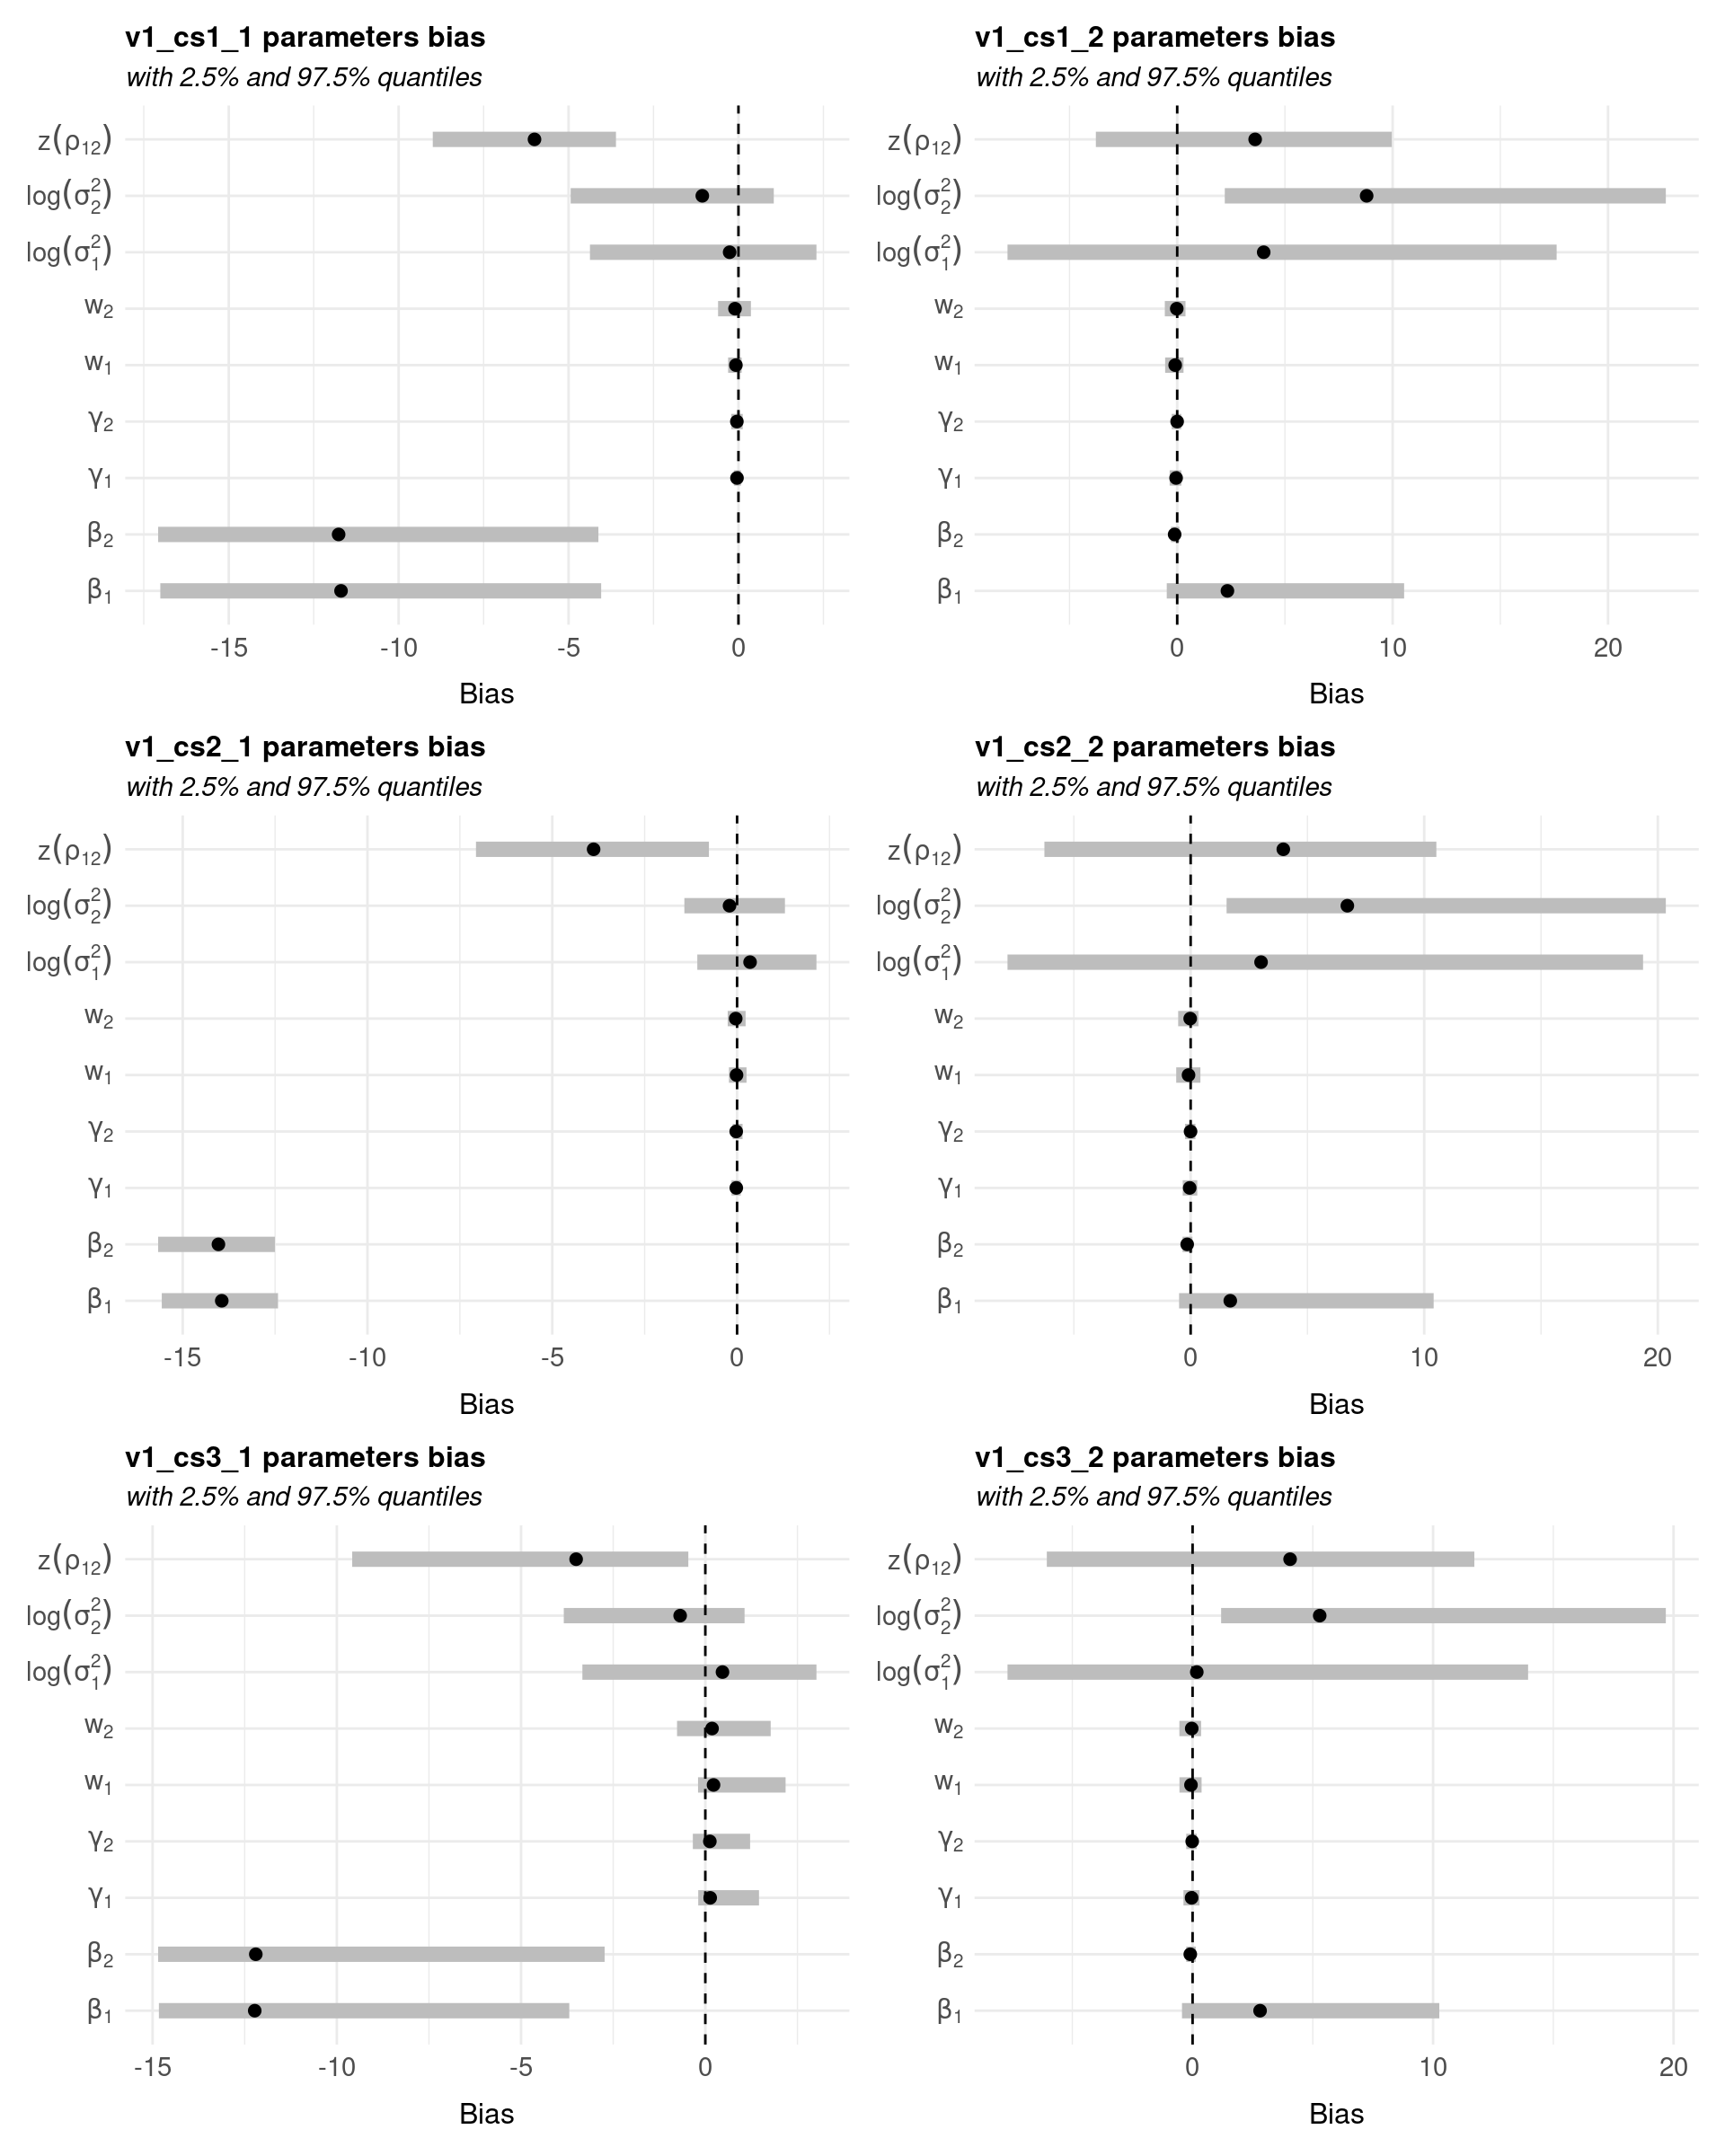
\includegraphics[width=\textwidth]{bias2plot-1.png}\\
 \begin{footnotesize}
  SOURCE: The author (2021).
 \end{footnotesize}
 \label{fig:bias2plot}
\end{figure}

\begin{figure}[H]
 \setlength{\abovecaptionskip}{.0001pt}
 \caption{PARAMETERS CORRELATION}
 \vspace{0.2cm}\centering
 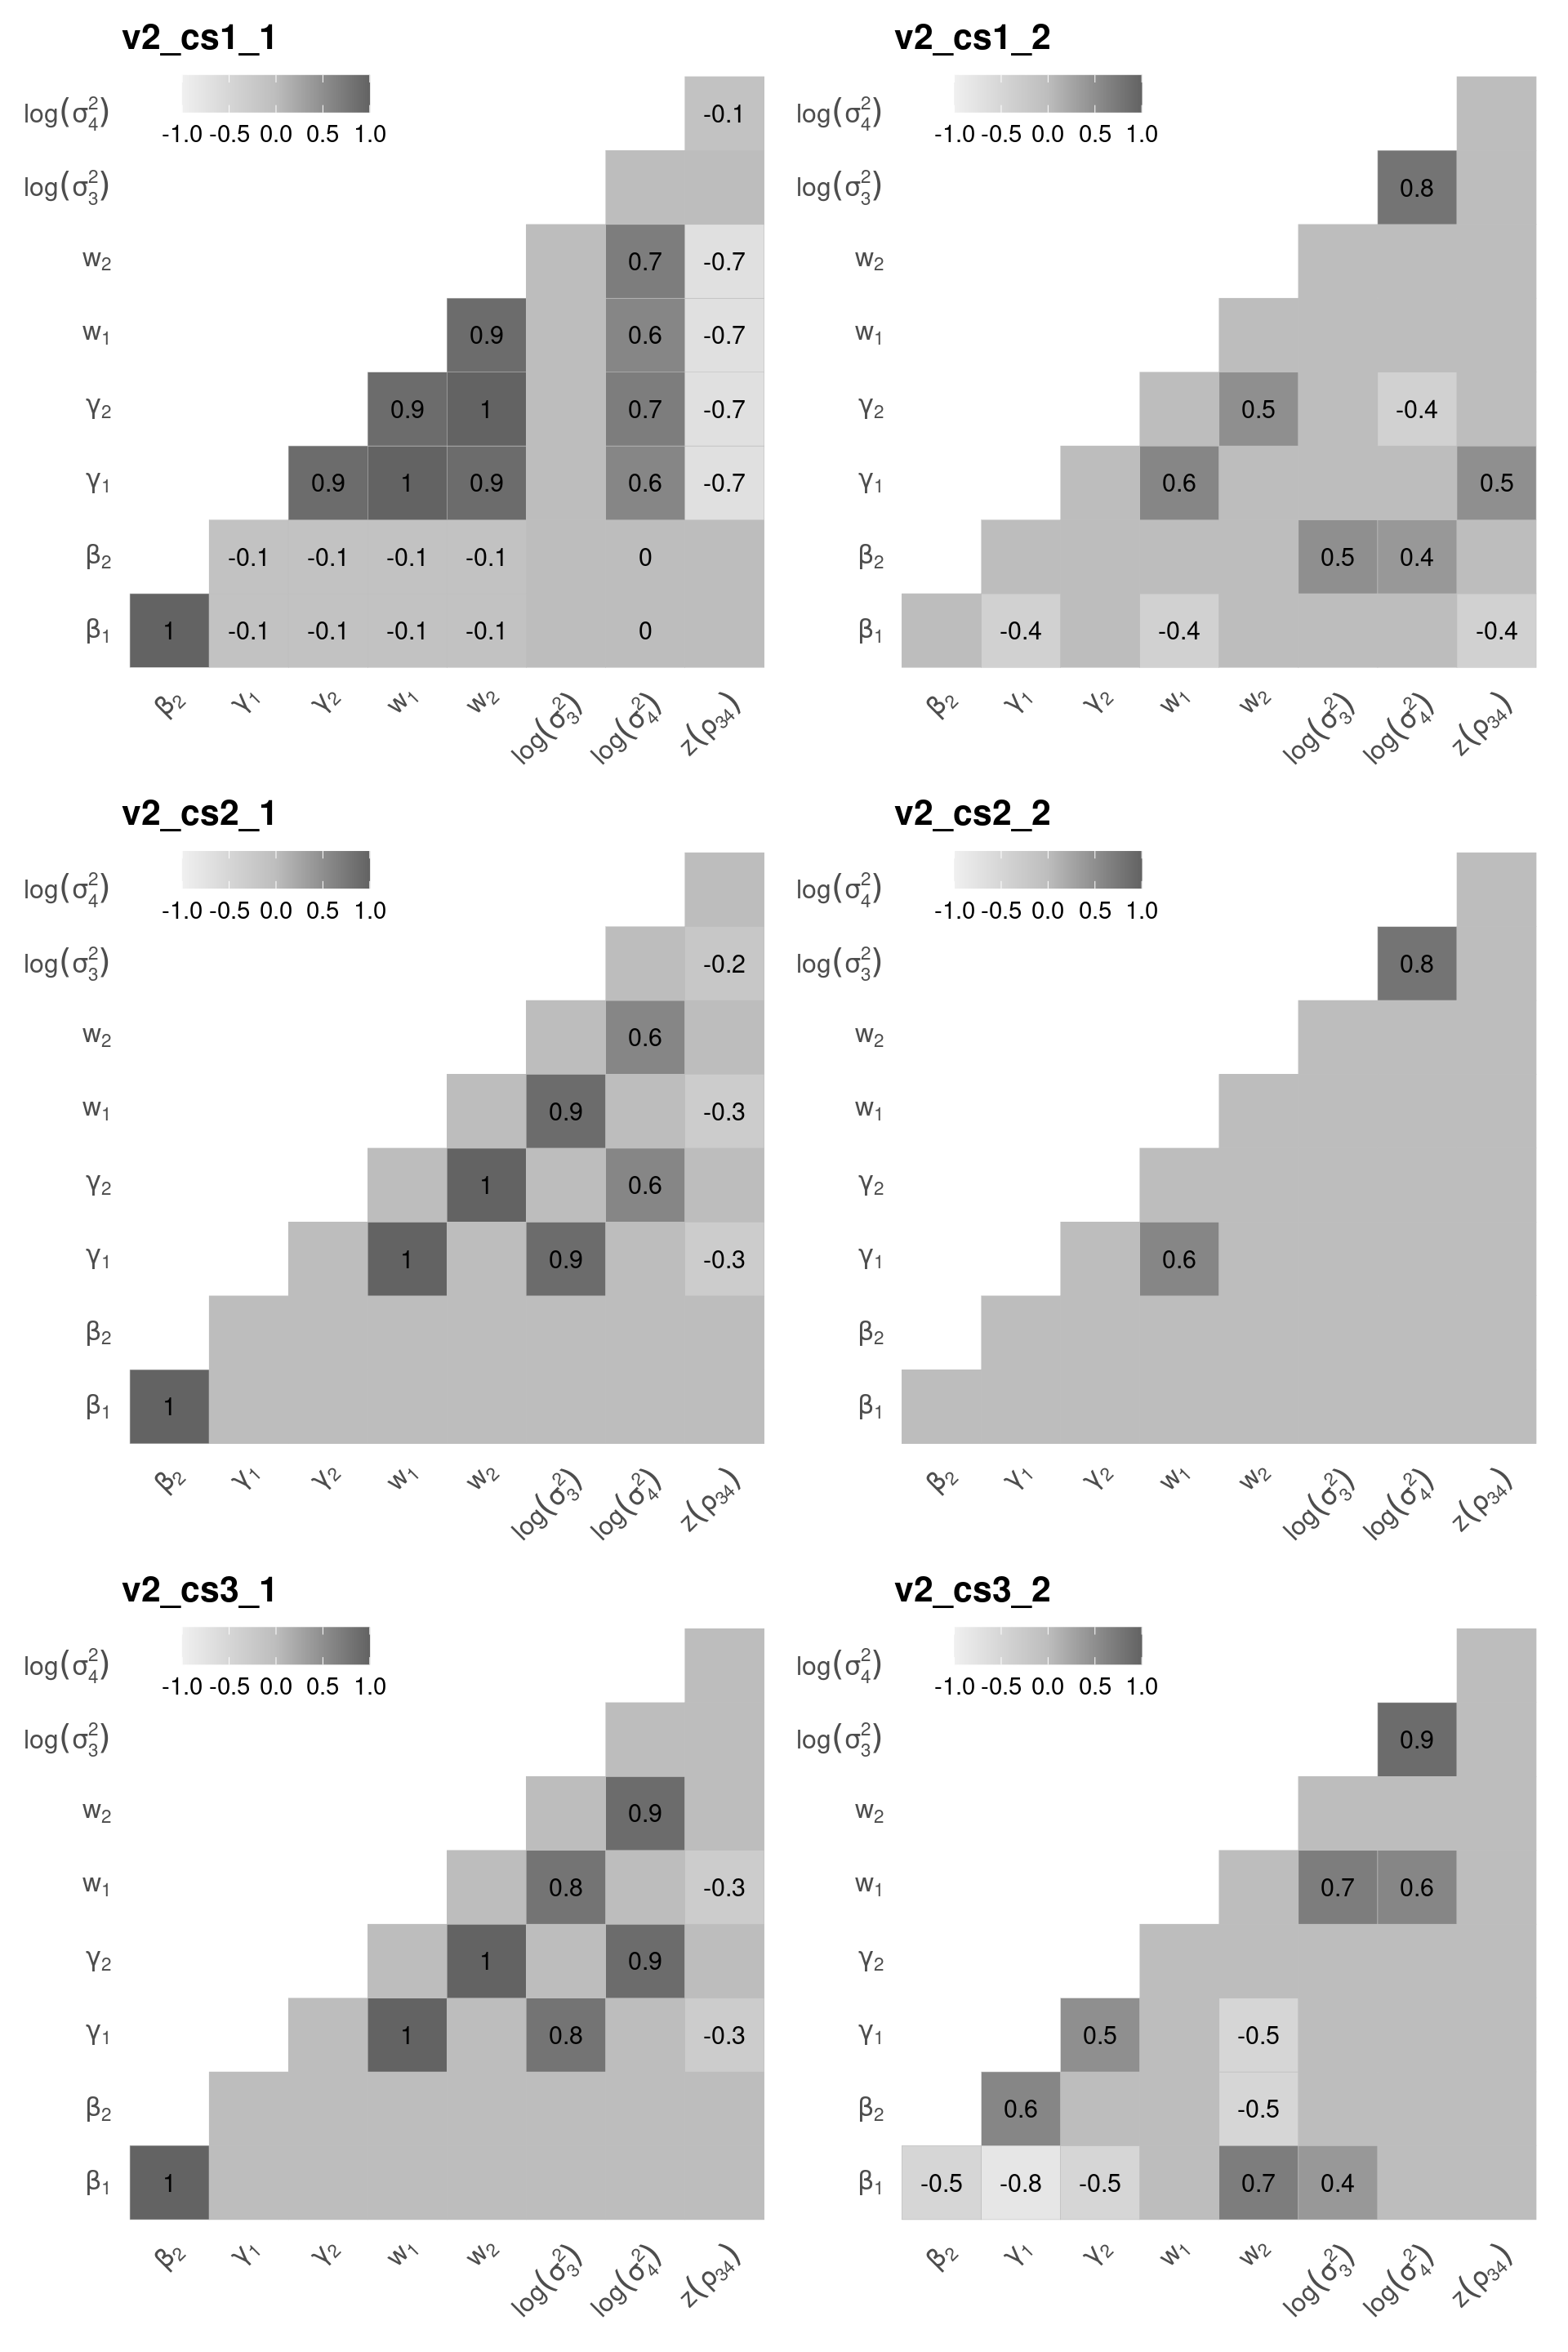
\includegraphics[width=\textwidth]{cor2plot-1.png}\\
 \begin{footnotesize}
  SOURCE: The author (2021).
 \end{footnotesize}
 \label{fig:cor2plot}
\end{figure}

\begin{figure}[H]
 \setlength{\abovecaptionskip}{.0001pt}
 \caption{VARIANCE-COVARIANCE MATRIX UPPER-TRIANGULAR COMPONENTS}
 \vspace{0.2cm}\centering
 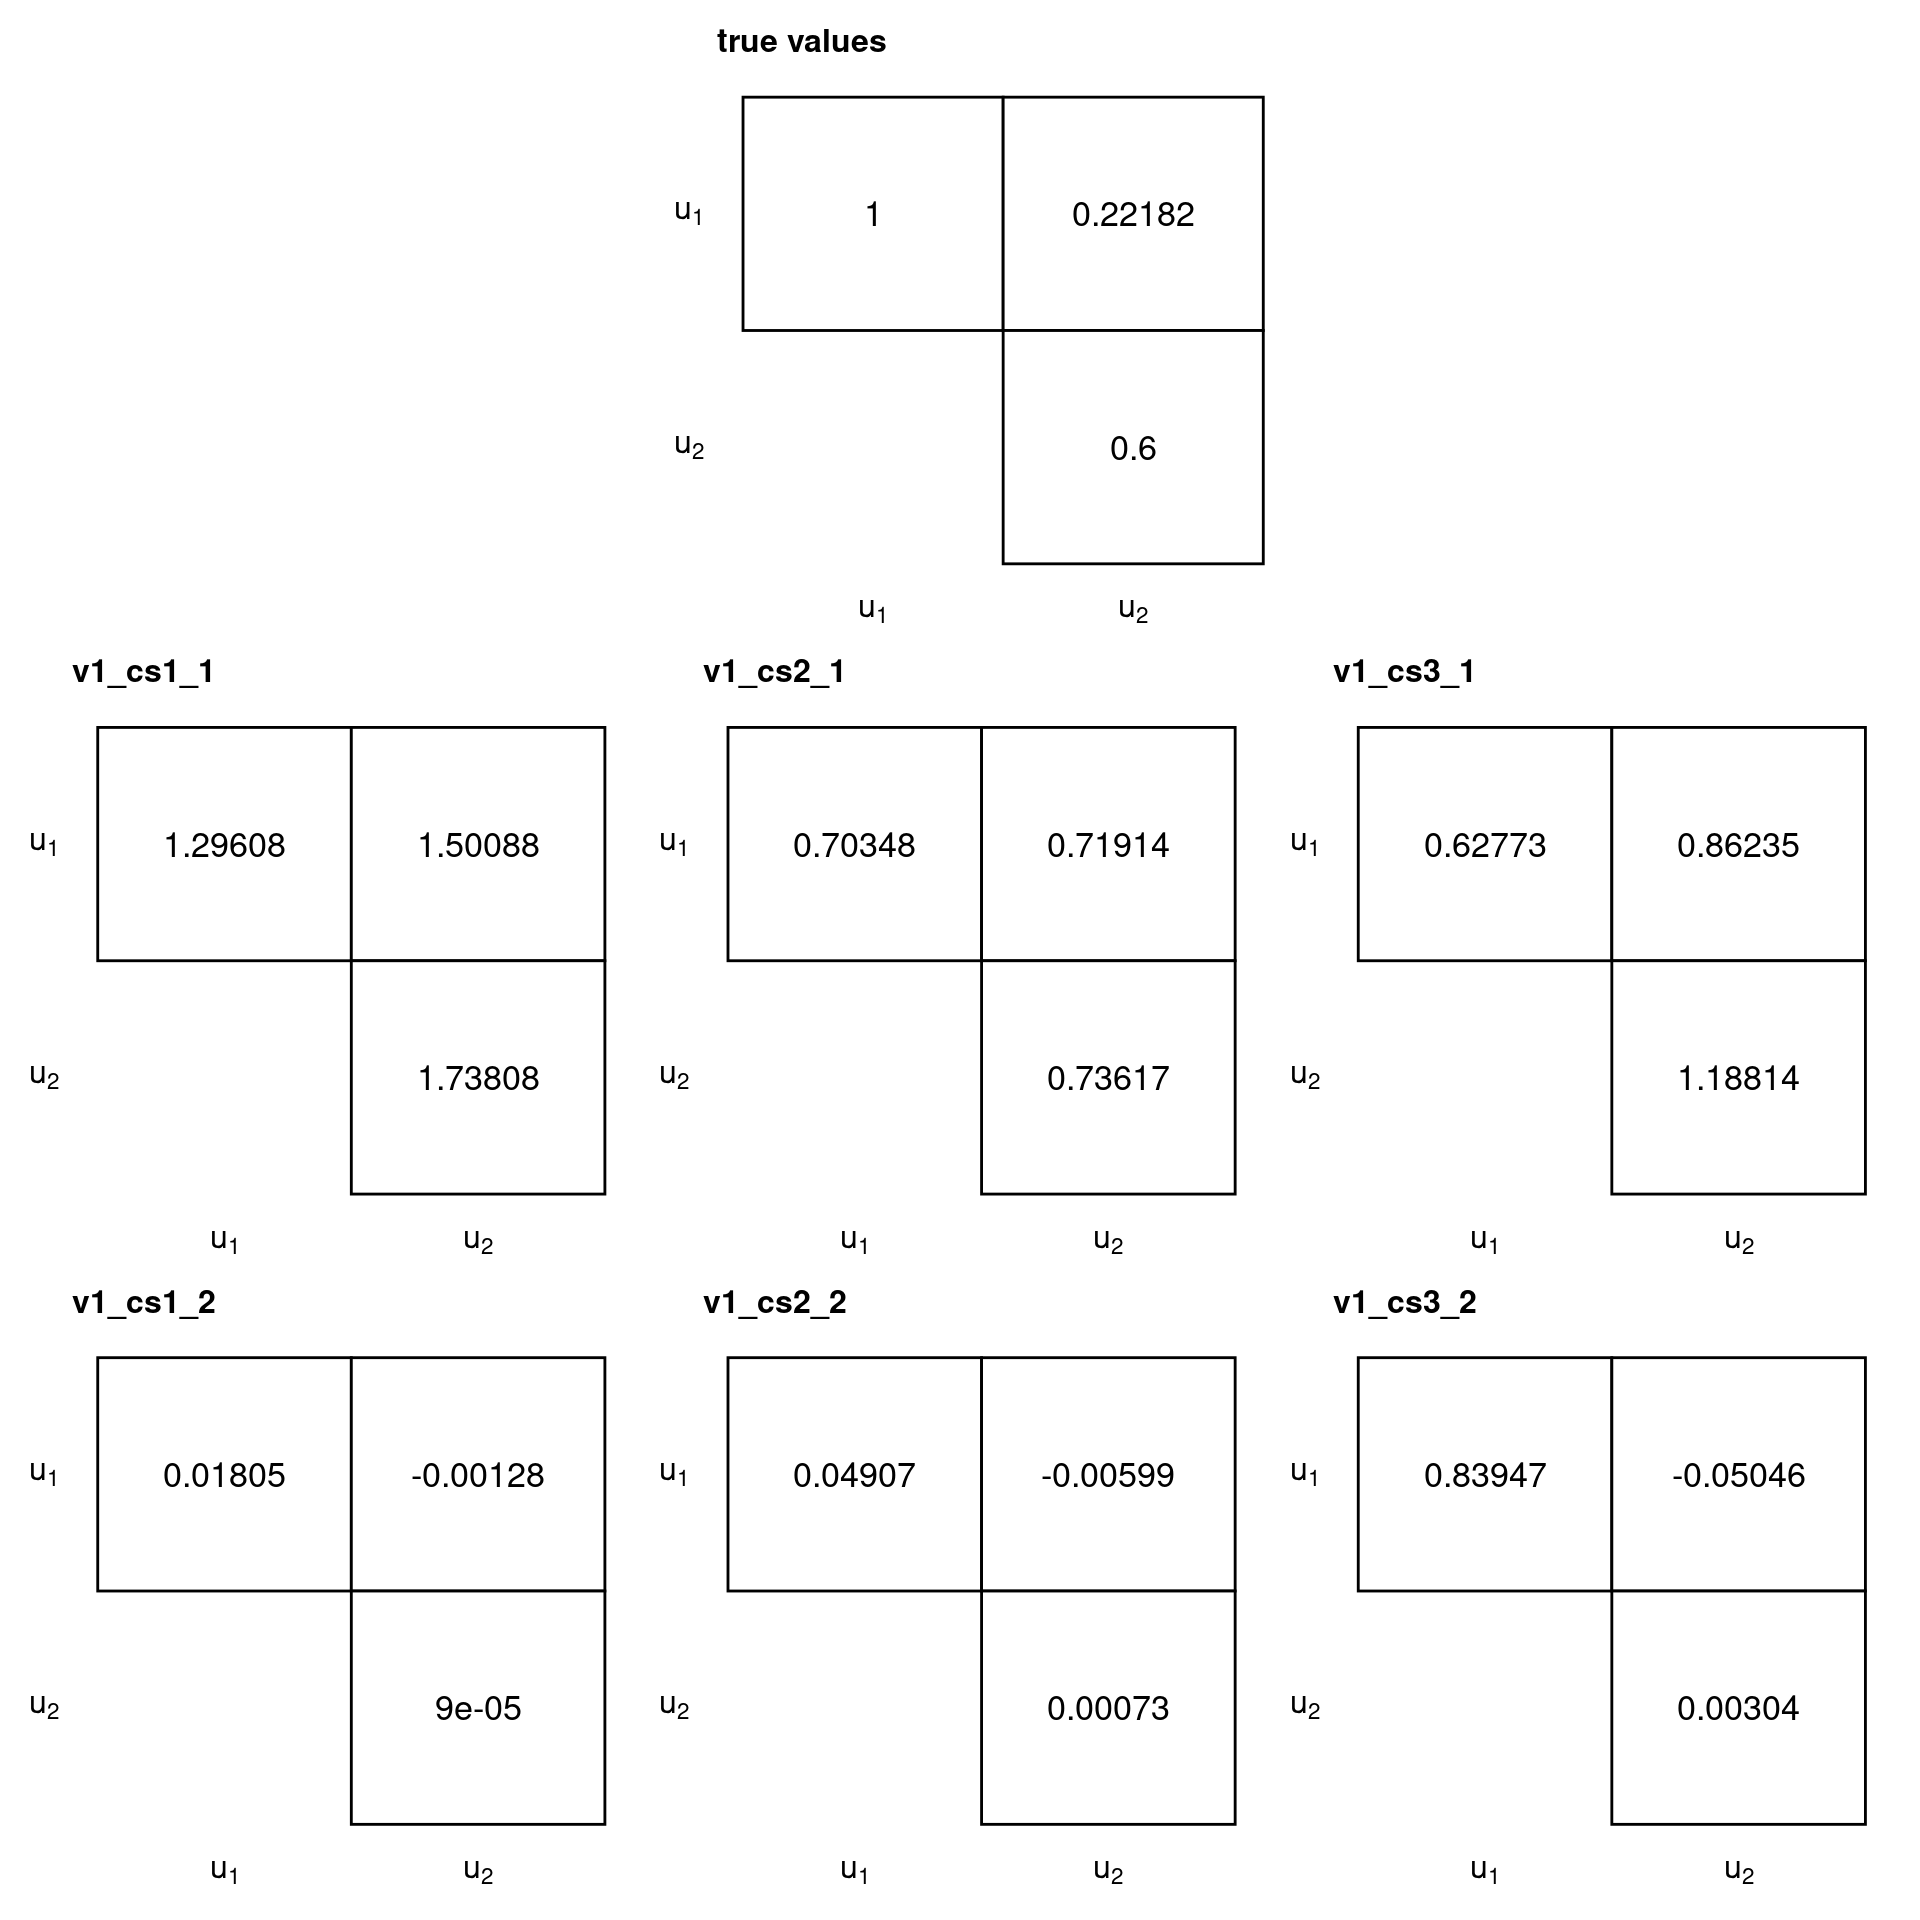
\includegraphics[width=\textwidth]{vcovs-1.png}\\
 \begin{footnotesize}
  SOURCE: The author (2021).
 \end{footnotesize}
 \label{fig:vcovs}
\end{figure}

\begin{figure}[H]
 \setlength{\abovecaptionskip}{.0001pt}
 \caption{CIFs}
 \vspace{0.2cm}\centering
 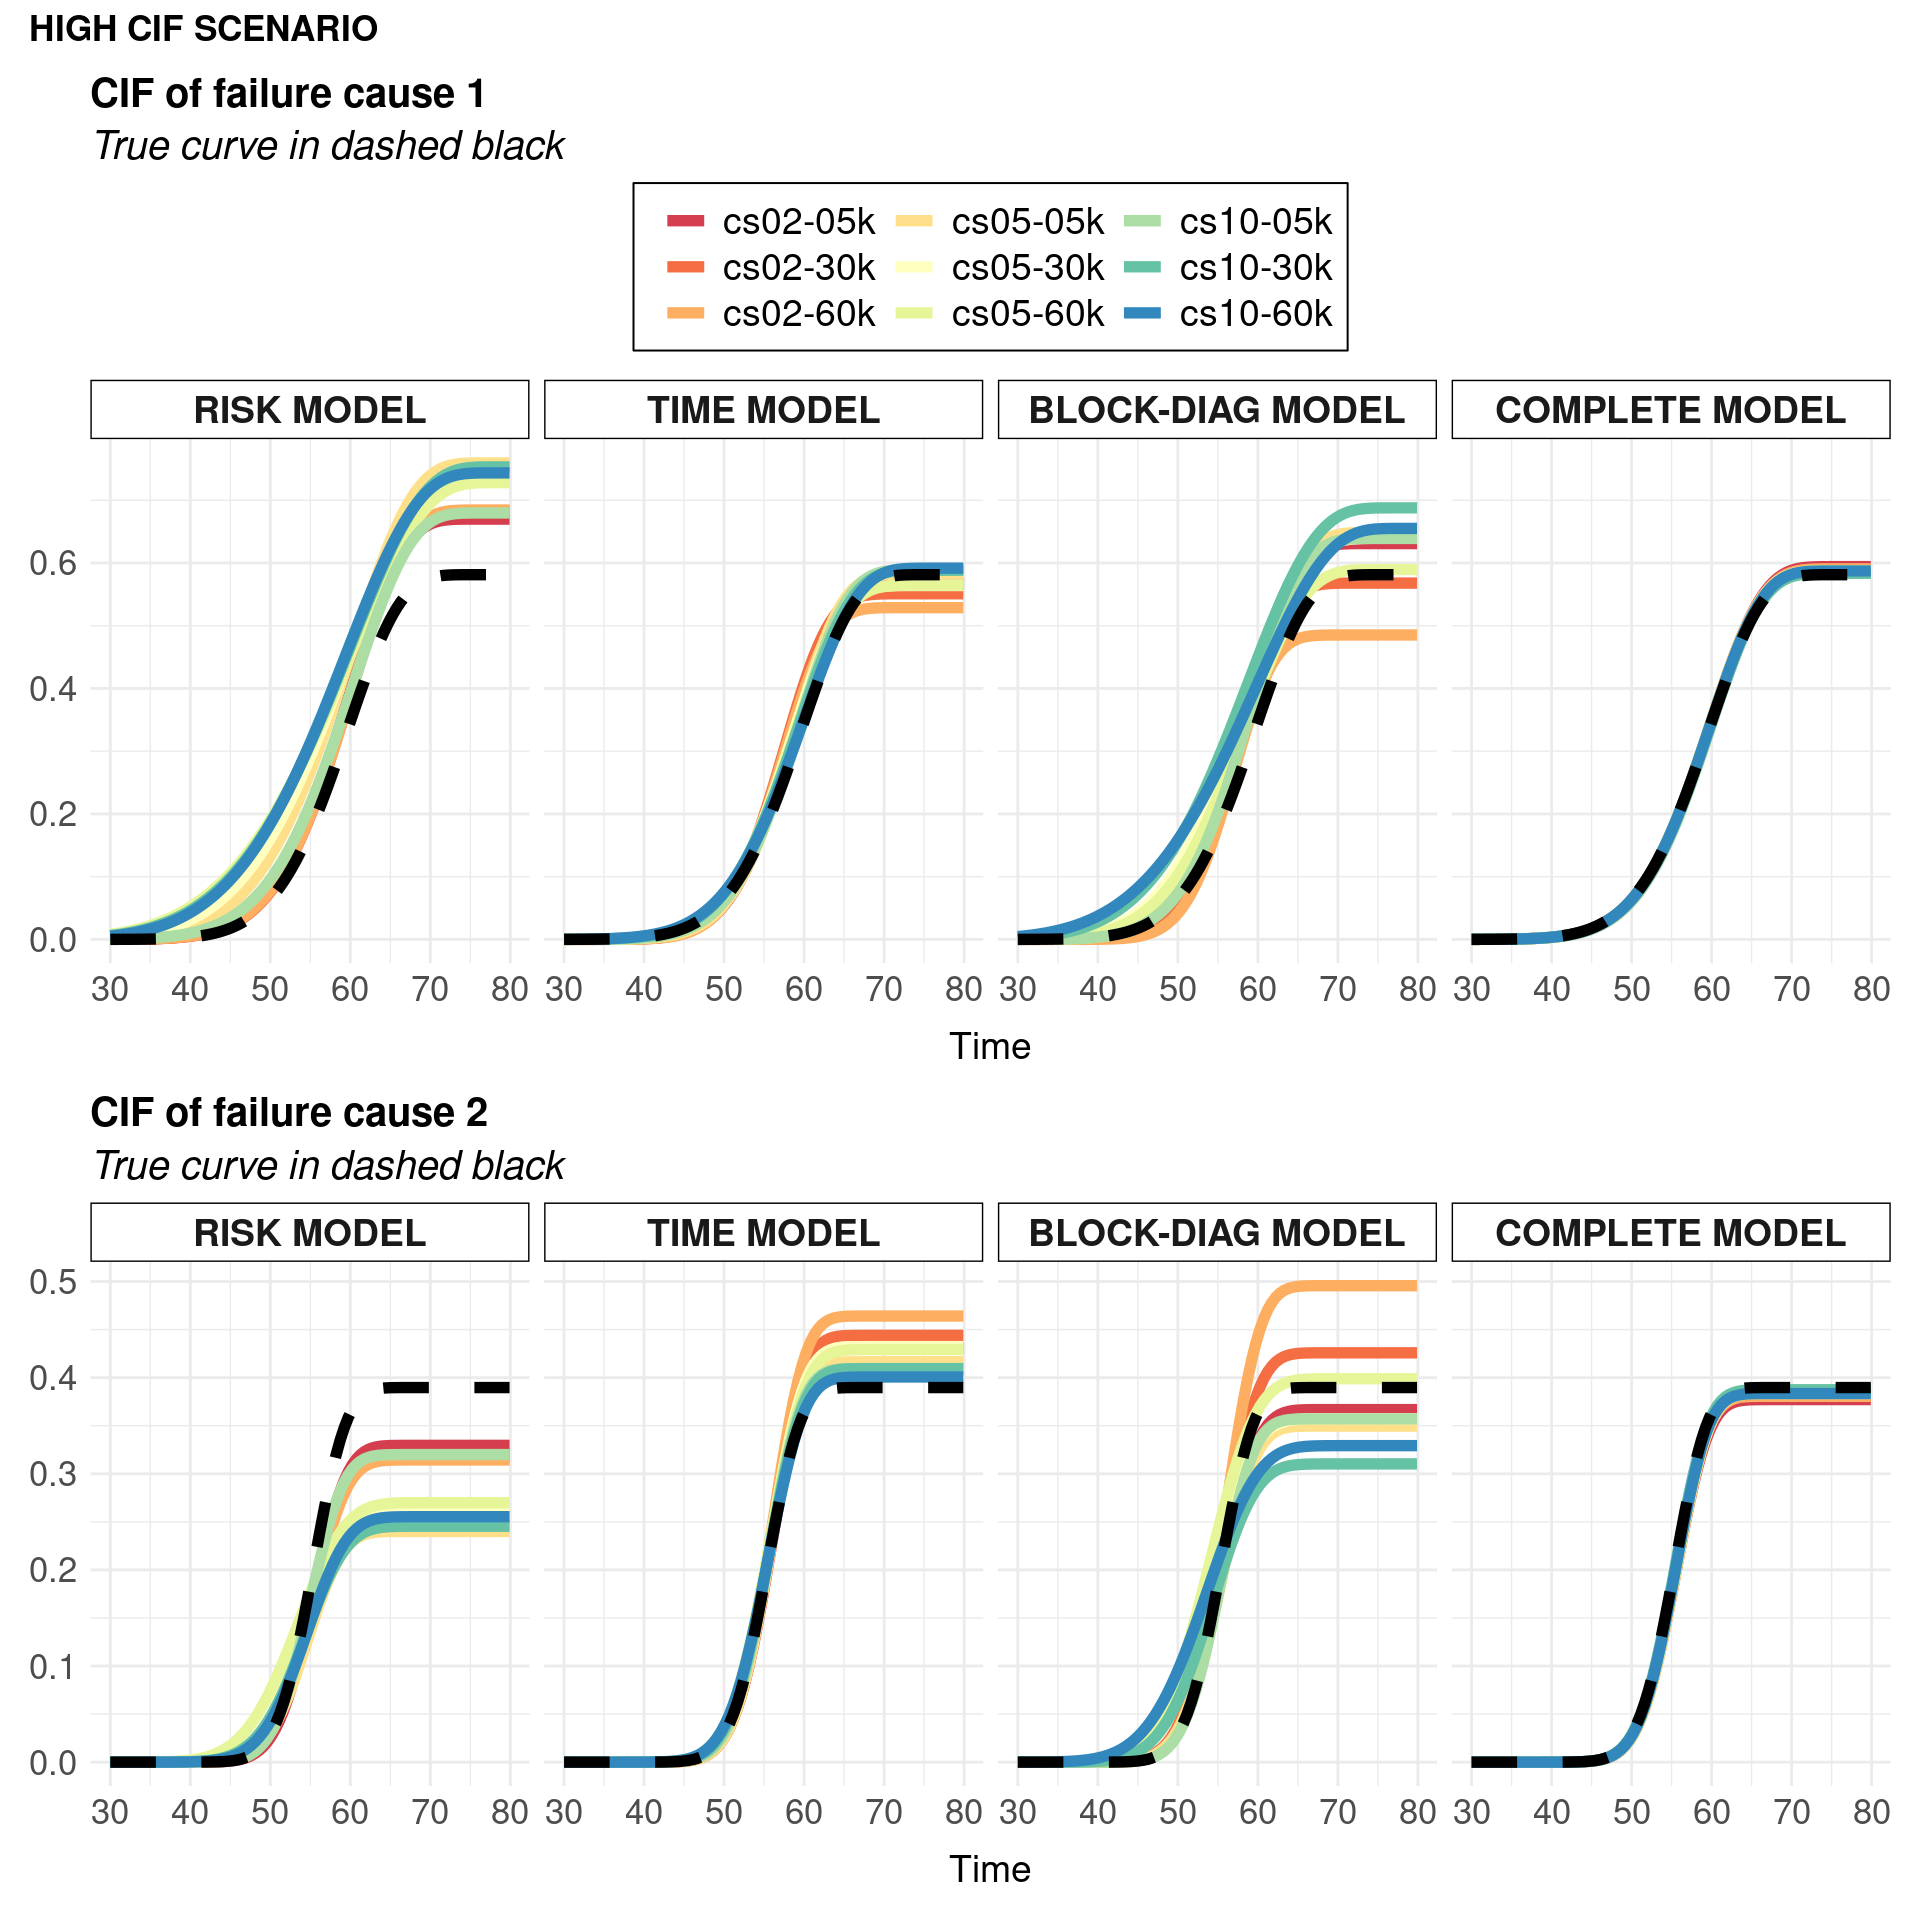
\includegraphics[width=\textwidth]{cifs-1.png}\\
 \begin{footnotesize}
  SOURCE: The author (2021).
 \end{footnotesize}
 \label{fig:cifs}
\end{figure}

\section{REAL-BASED DATASET}
\label{cap:datares}

% END ==================================================================
